\documentclass[Lau, oneside]{sapthesis}%remove "english" for a thesis written in Italian
\graphicspath{ {images/} }
%Bachelor's (laurea triennale) thesis : Lau 
%Master's (laurea specialistica) thesis: LaM 
%PhD's thesis: PhD 
\usepackage[italian]{babel} %use this package for a thesis written in Italian
\usepackage[utf8]{inputenx}
\usepackage{indentfirst}
\usepackage{microtype}
%\usepackage{chemformula}
%\usepackage{setspace}
%\usepackage{yfonts,color}https://www.overleaf.com/project/5e4187442ef81c00013a37ea
%\usepackage{siunitx}
%\usepackage{comment}
%\usepackage{multirow}
%\usepackage{varioref}
%\usepackage[bottom]{footmisc}
\usepackage{wrapfig}
\usepackage{float}
%\usepackage{type1cm}
\usepackage{lettrine}
\usepackage{caption}
\usepackage{subcaption}
\usepackage{bookmark}
%portare linespread a 1.1-1.3
\linespread{1.4}
%\usepackage{chngcntr}
\usepackage[nottoc, notlof, notlot]{tocbibind}
%\onehalfspacing
%\counterwithout{footnote}{chapter}
\usepackage{hyperref}
\hypersetup{
			hyperfootnotes=true,			
			bookmarks=true,			
			colorlinks=true,
			linkcolor=red,
                        linktoc=page,
			anchorcolor=black,
			citecolor=red,
			urlcolor=blue,
			pdftitle={Sviluppo App},
			pdfauthor={Edoardo Gabrielli},
			pdfkeywords={thesis, sapienza, roma, university}
 }

\title{Sviluppo App}
\author{Edoardo Gabrielli}
\IDnumber{1693726}
\course[]{Informatica}
\courseorganizer{Facolt\`a di Ingegneria dell’Informazione, Informatica e Statistica}
\submitdate{2019/2020}
\copyyear{2020}
\advisor{Prof. Emanuele Panizzi}
\authoremail{gabrielli.1693726@studenti.uniroma1.it}
\examdate{23 marzo 2020}
\examiner{Prof.}

%we refer to http://ctan.mirrorcatalogs.com/macros/latex/contrib/sapthesis/sapthesis-doc.pdf for an exhaustive description of the sapthesis documentclass.


\begin{document}

\frontmatter
\maketitle

\tableofcontents

\mainmatter
\chapter{Introduzione}
\label{ch:1}

\section{InfoStud e InfoProf}
\label{sec:pres}
L'app InfoStud nasce \textit{n} anni fa dalla necessità degli studenti di avere il sistema InfoStud sviluppato da InfoSapienza su mobile.
Data la natura poco \textit{mobile-friendly} del sistema web, nacque l'app ufficiale sotto il brand di SapienzaApps.

SapienzaApps, sotto il coordinamento del Prof. Emanuele Panizzi, pubblica e mantiene progetti come SeismoCloud e GeneroCity all'interno
del Gamification Lab.

InfoStud è l'app che si rivolge unicamente agli studenti iscritti alla Sapienza e mette a disposizione un parco di funzionalità ampio
che copre le funzioni standard del sistema padre (come visualizzazione e gestione esami) e andando oltre in alcuni casi: il sistema
di gestione dell'orario didattico semi-automatico, la compilazione dei bollettini automatica, la prenotazione dei posti in biblioteca, ecc.

InfoProf, al contrario, è l'app che si rivolge ai professori della Sapienza e vuole essere uno strumento alternativo, e più intuitivo, 
del sistema web. La semplicità di utilizzo dell'app va però analizzata e progettata in modo empirico. Questo studio porta via molto tempo 
al lavoro ed è per questo che gran parte della progettazione si traduce in prototyping e test di usabilità, con eventualmente molteplici
iterazioni. Lo stato dell'arte attualmente è un'app che permette di verbalizzare gli studenti, attivare gli OPIS e cercare le aule.
Queste funzionalità hanno un denominatore in comune: sono casi d'uso in cui l'utente potrebbe non avere il computer quando ha bisogno
di utilizzarle. La verbalizzazione infatti può essere fatta subito dopo un orale, senza dover aspettare di tornare in ufficio e 
registrare i voti di tutti gli studenti. L'OPIS, date le ultime disposizioni, deve essere attivato durante la lezione, ma un utente
potrebbe non voler portare un computer in aula solo per attivare il codice OPIS.

Il mio tirocinio, in larga parte, è stato composto dall'aggiunta di piccole funzionalità richieste dall'utenza o dalla risoluzione di 
problemi: su InfoStud mi sono occupato di migliorare il login, aggiungere un'icona su SmartBiblio per indicare i posti non gestiti
dal sistema, migliorare la dark-mode e aggiungere l'immagine del profilo nel menù laterale. Su InfoProf invece ho lavorato alla
traduzione automatica, anche qui sul login, sul date-picker nella registrazione del voto di un esame e infine sul vero protagonista del 
tirocinio, ovvero l'apertura di un verbale, in cui ho fatto uno studio più approfondito di cui parlerò in \ref{ch:3}.

\section{Perché?}
\label{sec:why}
%trovare articoli scientifici in merito. 
Lo smartphone è ormai uno strumento radicato nella nostra quotidianeità. Sono innumerevoli i modi in cui ha cambiato la nostra vita e la
produttività è uno degli aspetti centrali. Nel settore pubblico l'evoluzione dei sistemi informatici però pecca di una rigorosa analisi 
e progettazione, il che comporta perdite di tempo e difficoltà nell'utilizzo.
Dall'indagine preliminare che ho svolto infatti emerge che alcuni intervistati trovano l'interfaccia web \textit{error-prone}, mentre 
un professore assunto recentemente, ha dichiarato che la piattaforma non è affatto user-friendly e che la logica vorrebbe che ci fosse
un tasto "crea appello", non che debba andarlo a cercare in "verbalizzazione". Anche all'interno del team di sviluppo, quando ci è
stata presentata per la prima volta l'interfaccia, abbiamo faticato a capire come svolgere i task che un professore è tenuto normalmente
a fare. Tolti errori grossolani come l'assegnazione di termini differenti alla stessa cosa [trovare un termine più adatto] 
\textbf{(inserire figura)}, esistono delle criticità che vanno contro la logica comune: se andiamo ad osservare la lista degli insegnamenti,
alla destra di ogni elemento possiamo osservare un numero che rappresenta il numero di \textit{corsi} selezionati accoppiati con quell'
insegnamento. Se selezioniamo il checkbox dell'elemento e andiamo all'interno del sotto-menù, deselezionando tutti i corsi, l'insegnamento
rimarrà selezionato. Una buona interfaccia \textbf{(citare)}, invece, dovrebbe aiutare l'utente ad evitare gli errori.

%citare le statistice del miur riguardo età e numero di docenti della sapienza

%L'approccio che ho avuto quindi è stato quello di capire cosa gli utenti ritengono più importante nell'apertura di un verbale e mettere
%in secondo piano le funzionalità che vengono usate raramente. Vedremo infatti che paradossalmente l'interfaccia web, ai docenti che 
%hanno imparato ad usarla, piace.


\chapter{Metodologie di sviluppo}
\label{ch:2}

\section{Organizzazione}
\label{sec:team}
Il team è composto da studenti impiegati nello sviluppo per circa tre mesi. E' prassi iniziare ad ambientarsi nei progetti attraverso
l'attività di bug-fixing: familiarizzare con il codice e con i colleghi è centrale dato che per molti di noi è la prima esperienza
dentro un progetto di discrete dimensioni e all'interno di un contesto semi-professionale.

La metodologia di sviluppo che si adatta meglio alle nostre esigenze è l'Agile, il quale si basa su un insieme di regole il cui senso
generale è un approccio adatto ai cambiamenti, non fisso e rigoroso, che misura i progressi attraverso codice funzionante e incoraggia 
il rilascio continuo del software per soddisfare l'utente finale. 

Un aspetto fondamentale che si ricollega a questo è l'integrazione
continua del codice prodotto dagli sviluppatori: nel laboratorio utilizziamo GitLab, un sistema di controllo versione che tiene
traccia delle modifiche, segnala i conflitti che possono generarsi dalla modifica simultanea dello stesso file e aiuta a gestire i compiti 
del singolo sviluppatore.
Ad ogni \textit{merge request}, le modifiche apportate al codice sono revisionate da un controllo umano che garantisce la qualità del codice.
Se infatti lo stile non è coerente con il resto del progetto, se ci sono bug introdotti dalle modifiche o altri problemi, la merge request 
viene respinta.

\section{Tecnologie utilizzate}
\label{sec:tech}
Per sviluppare il front-end delle app utilizziamo Ionic Framework v3, che è basato su AngularJS. Ionic permette di utilizzare tecnologie
web per creare interfacce secondo gli standard di Android e iOS. Il vantaggio dell'uso di Angular è che il codice non va adattato ad alcuna
piattaforma, inoltre per chiunque abbia già una discreta conoscenza della programmazione web è immediato iniziare a programmare. Tutto
ciò velocizza molto la scrittura di una UI, ma bisogna fare dei compromessi: l'interfaccia non segue diligentemente gli standard imposti
dal Material Design o dall'iOS UI Design perché deve adattarsi ad entrambe le piattaforme. Un'altra criticità è che di fatto l'app è
un'interfaccia web con caratteristiche \textit{app-like}, ovvero una Progressive Web App sviluppata in Angular. 
Il ruolo di Ionic è fornire gli elementi dei vari standard di design già fatti e di integrare anche le funzionalità native attraverso
Ionic Native o Cordova. Ciò significa che le prestazioni ne risentono ripetto ad un'app nativa. Inoltre ad oggi Ionic è alla versione 5,
ma è impossibile aggiornare i progetti senza andare a creare dei conflitti che vanno risolti manualmente, vista la mole di codice che è
stato scritto quindi, siamo costretti a rimanere ad una versione di qualche anno fa, all'occorenza programmando manualmente le novità
introdotte dagli standard.

InfoStud ed InfoProf sono progettati seguendo un pattern architetturale loro. L'idea generale è quella di tenere separate le responsabilità
di ogni componente. Ciò si traduce sinteticamente in:

\begin{itemize}
	\item Model: rappresentano le classi, contiengono i dati dell'applicazione a cui si accede attraverso i metodi che forniscono;
	\item View: la view accede ai dati forniti dai modelli e li presenta all'utente, inoltre comunica con i controller e i provider;
	\item Controller: il controller risponde alle azioni dell'utente intercettate dalla view e si occupa soltanto della logica di business, a volte comunica con i provider;
	\item Provider: di fatto "fornisce" i dati. Ha il compito di utilizzare le API e consegnare i dati alla view attraverso i model.
\end{itemize}

\begin{figure}[ht]
	\caption{Schema del funzionamento del pattern utilizzato da InfoStud e InfoProf.}
	\centering
	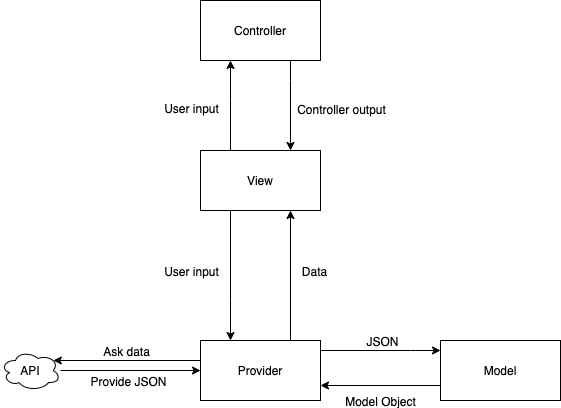
\includegraphics[width=0.8\textwidth]{arch-pattern-img}
	\label{fig:pattern}
\end{figure}

I vantaggi dell'utilizzo di questo modello è quello di separare la logica di presentazione, quella di business e quella di accesso ai dati
in entità distinte tra loro in modo da favorire il lavoro di gruppo. Inoltre, essendo Angular un framework che impone una separazione in moduli del codice [citare], una divisione
così fatta incoraggia il riuso del codice ovviamente. %fare diagramma di sequenza e un esempio

%Tra ch 1 e 2 bisognerebbe aggiungere altre 8 pagine, magari apliare la descrizione delle issues


\chapter{Progettazione}
\label{ch:3}
%inserire diagramma di flusso di come viene fatta la progettazione (nf -> prototyping -> test -> repeat)
L'attività di progettazione consiste nel trovare i bisogni dell'utente attraverso delle domande rivolte agli stessi, costruire un prototipo che rispecchi ciò che è emerso dalle domande, eseguire dei test di usabilità sul prototipo e, a seconda delle criticità, emerse dai test modificare il prototipo e ripetere i test finchè si è trovata un'interfaccia che funzioni per gran parte degli utenti.

\section{Need-finding}
\label{sec:nf}
La prima cosa che ho fatto è capire quali sono i bisogni dell'utente. Non avendo mai utilizzato InfoStud docenti, il primo approccio al sistema è stato insieme al Prof. Panizzi che mi ha mostrato il processo di apertura di un verbale d'esame, le varie funzionalità già esistenti e i dati richiesti nel form che il docente è tenuto a compilare. Da questa dimostrazione sono emerse delle criticità: per un utente inesperto come me è difficile prendere confidenza con l'interfaccia in quanto spesso vengono utilizzati diversi termini per rappresentare lo stesso concetto, c'è una lista molto grande di insegnamenti da poter selezionare e bisogna prestare attenzione a quali sono quelli che si selezionano perchè in alcuni casi il sistema potrebbe restituire un errore. Inoltre l'interfaccia non spiega come inserire il giorno dell'esame (quello che effetivamente gli studenti vedono in fase di prenotazione), bisogna chiederlo a chi già ne è a conoscenza.

Essendomi fatto un'idea delle criticità dell'interfaccia attuale, ho creato un sondaggio inviando via email le seguenti domande:

\begin{enumerate}
	\item Se tiene più di un corso, preferisce aprire un verbale unico o aprirne uno per ogni corso che tiene? 
	\item Trova confusionario il processo di apertura di un verbale? Perché?
	\item Quanto tempo prima dalla data dell’esame apre il verbale?
	\item Quanto tempo dà agli studenti per prenotarsi?
	\item E quanti giorni prima, dal giorno dell’esame, chiude le prenotazioni? 
\end{enumerate}

Il sondaggio ha solo una domanda aperta, tra l'altro opzionale, in quanto volevo rendere il sondaggio molto corto in modo da aumentare 
le possibilità di risposta. Per coloro che volessero dedicarmi più tempo ho invece chiesto di argomentare in modo da avere risposte
più complete, infatti a fine email ho incoraggiato ad argomentare le risposte il più possibile.

La prima domanda è stata fatta per capire come gestiscono la lista degli insegnamenti: la lista sull'app infatti è difficile da gestire
vista la sua lunghezza. Quindi se la maggior parte dei professori sceglie di selezionare tutto, potrei sintetizzarla in qualche modo.
La seconda ha un carattere generale, che mira a scoprire qualcosa di più da parte dell'utente.
Le domande dalla 3 alla 5 invece servono a capire se esistono dei vincoli nella scelta delle date per cercare di automatizzare il processo.

Gli intervistati sono 60, presi casualmente in vari dipartimenti dell'ateneo in modo di avere un campione più eterogeneo possibile.
I professori che hanno invece risposto sono stati 19.

\subsection{Verbale unico o uno per ogni corso?}

Come vediamo dall'immagine \ref{fig:d-i} la maggioranza degli intervistati preferisce aprire un verbale per ogni insegnamento. Ricordo che "un insegnamento", nella tabella, corrisponde a tutti gli insegnamenti vecchi che hanno cambiato nome e per ognuno esistono due righe: una per l'anno accademico corrente ed una per quello precedente.

\begin{figure}[H]
	\caption{Grafico delle risposte date alla prima domanda.}
	\centering
	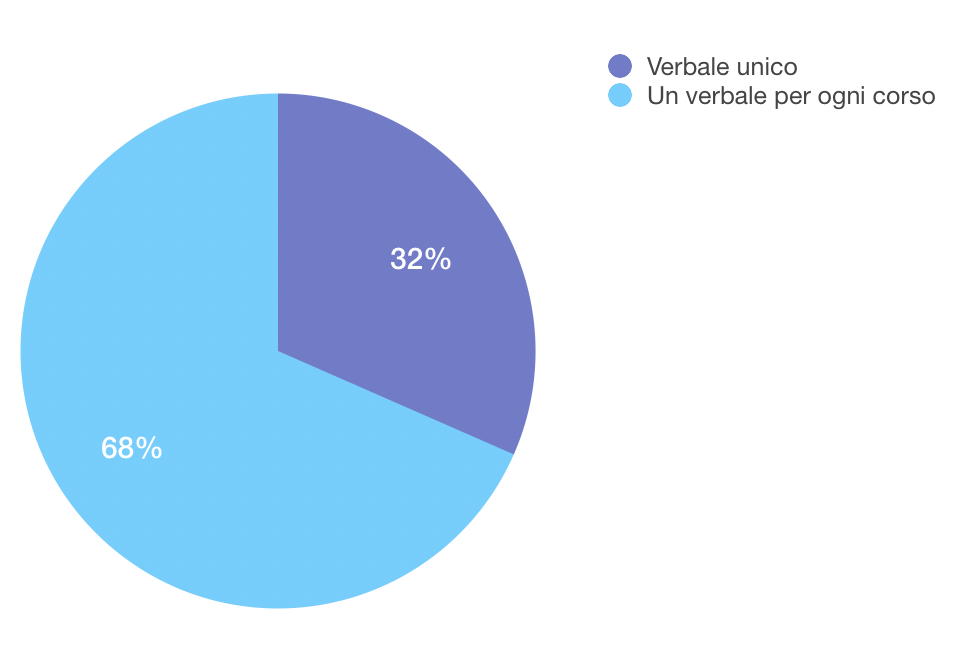
\includegraphics[width=0.6\textwidth]{d-i}
	\label{fig:d-i}
\end{figure}

\subsection{Trova confusionario il processo di apertura di un verbale?}
Qui i risultati sono un po' sorprendenti perchè la maggioranza sostiene che non ci siano grossi problemi, sebbene comunque una percentuale non trascurabile abbia risposto il contrario. Ciò potrebbe essere imputabile al fatto che per molti anni sono stati abituati a questo sistema ed hanno imparato ad utilizzarlo agevolmente, con degli escamotage. Uno fra tutti è quello di utilizzare la funzionalità del "Duplica appello", che di fatto copia un appello già creato. L'utente la utilizza per non dover selezionare nuovamente gli insegnamenti (cambiando solo le date e le note), ma il nome della funzionalità di fatto suggerisce un altro tipo di utilizzo. Vedremo in seguito come si è trovata una soluzione più elegante a questo problema.

Alcuni dei docenti che hanno risposto "no" alla domanda, si sono espressi anche sul perché. Cito: 
\begin{itemize}
	\item "Il processo di apertura di un verbale più che confusionario è piuttosto "error-prone" con campi che si riempiono automaticamente o campi che scompaiono quando si effettua una scelta da un menù a tendina."
	\item "Ho difficoltà a mettere gli appelli di esame perchè non so mai per quali corsi debba essere valido l'esame. E sovente gli studenti non vedono l'appello o meglio alcuni lo vedono e altri no."
	\item "La scelta degli insegnamenti è caotica perché ci sono nomi ripetuti con diverse diciture e lo stesso codice (non parliamo poi dei corsi di studio associati, che non apro neppure); l'anno accademico non serve a niente e complica l'immissione anche perché crea il refresh dell'elenco materie; oltre ad "avvisi e note" bisognerebbe poter inserire il luogo dell'esame e l'orario o i vari appelli, se più d'uno."
	\item "Un problema che trovo riguarda la scelta dell'A.A di riferimento. Vorrei che non esistesse questa opzione."
\end{itemize}

Ho avuto inoltre la fortuna di intervistare un docente nuovo, che mi ha esplicitamente detto che ha avuto grosse difficoltà nell'aprire il suo primo verbale. Nessuno gli ha spiegato come fare, dunque ha impiegato molto tempo a cercare le funzionalità che gli servivano.

\begin{figure}[ht]
	\caption{Grafico delle risposte date alla seconda domanda.}
	\centering
	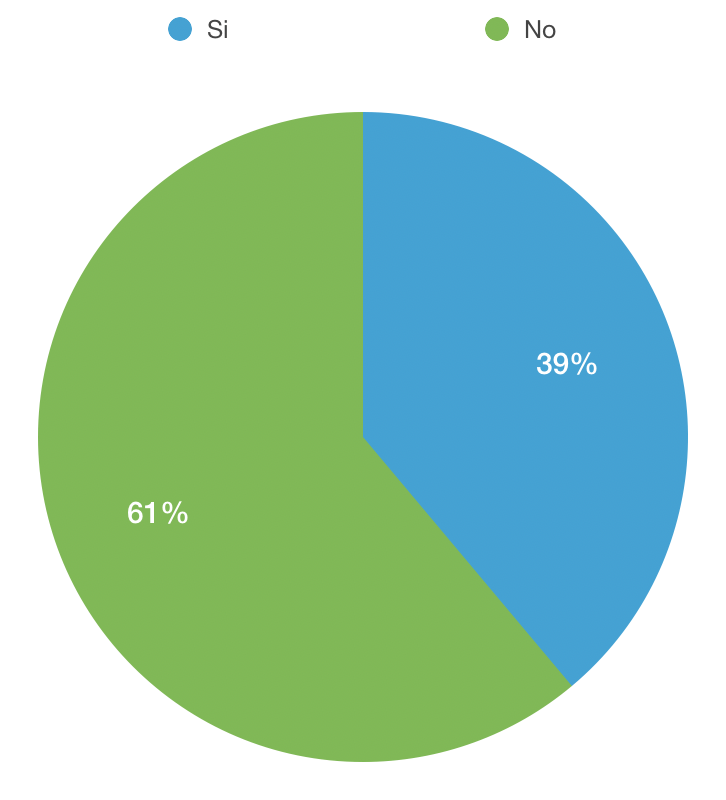
\includegraphics[width=0.4\textwidth]{d-ii}
	\label{fig:d-ii}
\end{figure}

\subsection{Quanto tempo prima dalla data dell’esame apre il verbale?}
La metà degli intervistati ha dichiarato di aprire i verbali all'inizio dell'anno accademico. Infatti molti dipartimenti impongono questa condizione ai docenti, dunque è necessario velocizzare il tempo di apertura di un singolo verbale perchè aprirne 7 per ogni insegnamento potrebbe essere un'attività che porta via del tempo.

\begin{figure}[ht]
	\caption{Grafico delle risposte date alla terza domanda.}
	\centering
	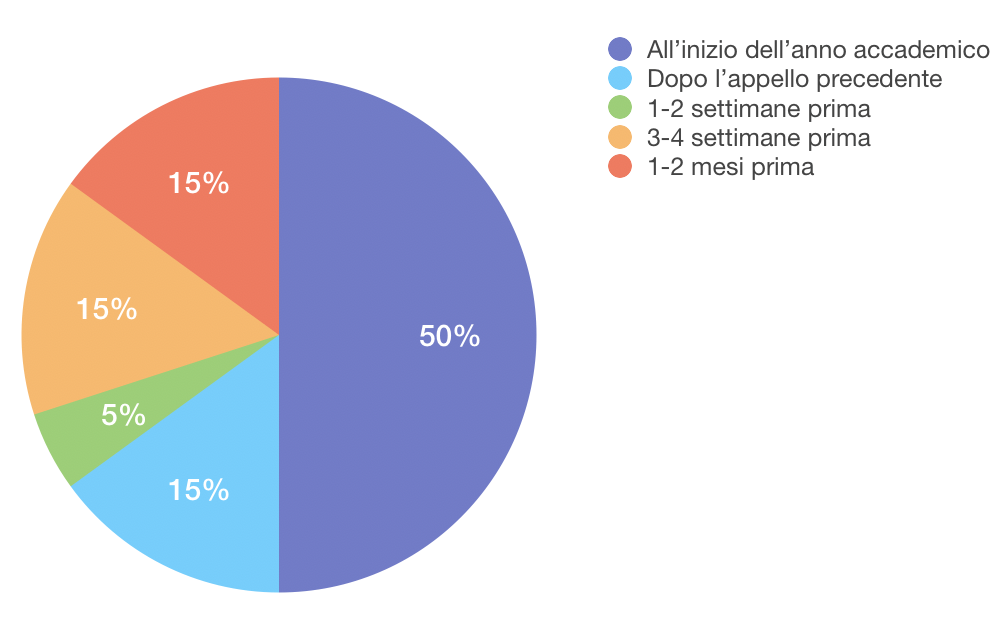
\includegraphics[width=0.8\textwidth]{d-iii}
	\label{fig:d-iii}
\end{figure}

\subsection{Quanto tempo dà agli studenti per prenotarsi?}
Qui le risposte sono piuttosto eterogenee.

\begin{figure}[ht]
	\caption{Grafico delle risposte date alla quarta domanda.}
	\centering
	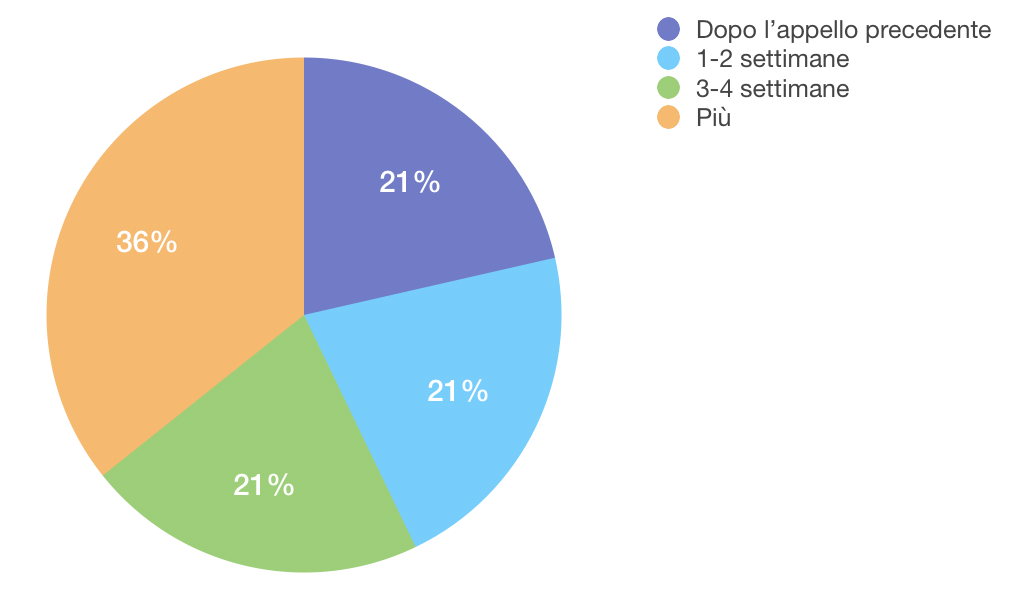
\includegraphics[width=0.8\textwidth]{d-iv}
	\label{fig:d-iv}
\end{figure}

\subsection{E quanti giorni prima, dal giorno dell’esame, chiude le prenotazioni? }
Al contrario invece, qui la maggior parte dei docenti preferisce chidere le prenotazioni 1 o 2 giorni prima dal giorno dell'esame. Questa è una buona notizia perchè in questo caso posso utilizzare l'informazione per definire un default per una futura funzionalità di compilazione automatica del form.
\begin{figure}[ht]
	\caption{Grafico delle risposte date alla quinta domanda.}
	\centering
	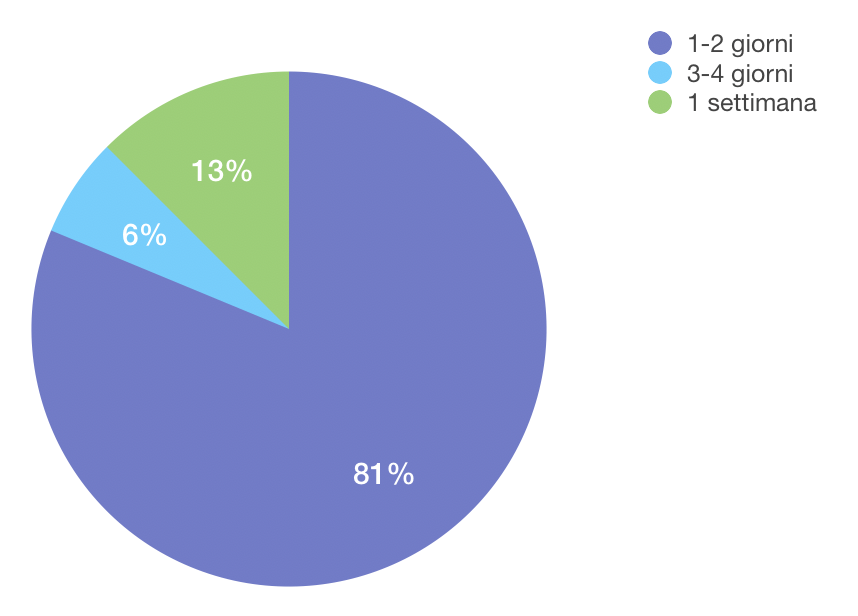
\includegraphics[width=0.7\textwidth]{d-v}
	\label{fig:d-v}
\end{figure}


\section{Requisiti}
\label{sec:req}
%citare "Developing SMASH", Nielsen e Gerhardt-Powals' cognitive engineering principles
Nella precedente sezione ho descritto le riposte che sono state date al sondaggio ed ho effetivamente trascritto quali sono i margini di miglioramento. Abbiamo visto che una buona percentuale dei partecipanti al sondaggio non è contenta dell'interfaccia desktop e mi ha dato dei buoni spunti su cui lavorare, come l'aggiunta di orario e luogo d'esame. Ma per ora mi concentrerò soltanto nel miglioramento dell'esperienza utente.

In questo capitolo descriverò i requisiti che ho individuato, per poi passare alle iterazioni che ho passato prima di arrivare all'interfaccia finale.

Requisiti \footnote{Non ordinati.}:
\begin{enumerate}
	\item L'ambiente in cui l'app funzionerà per la maggior parte del tempo è su uno smartphone, dunque su uno schermo molto piccolo rispetto a quello del PC. Quindi è necessario sintetizzare gli elementi che su InfoStud docenti occupano più spazio, come ad esempio la tabella degli insegnamenti.
	\item L'apertura di un verbale deve avvenire nel minor tempo possibile, in modo da velocizzare l'apertura consecutiva di più verbali.
	\item L'interfaccia deve aiutare l'utente ad evitare gli errori o perlomeno dare delle informazioni chiare quando se ne commette uno.
	\item L'interfaccia dovrebbe essere ragionevolmente semplice da capire ed utilizzare, senza perdere troppo in precisione \footnote{Per precisione intendo la quantità di informazione fornita all'utente, comparata all'interfaccia desktop.} e senza aver bisogno di una spiegazione.
\end{enumerate}

\section{Iterazioni}
%parlare solo dei prototipi e fare una valutazione secondo test/euristiche a fine di ogni iterazione.
\subsection{Valutazione dell'interfaccia}
%parlare di euristiche e test
Prima di cominciare a parlare di della fase di prototyping, introduco le tecniche di valutazione dell'interfaccia che ho utilizzato. Le tecniche di valutazione testano l'usabilità e le funzionalità di un sistema, in modo da valutarne i problemi e gli effetti che l'interfaccia ha sull'utente. Queste tecniche inoltre richiedono un artefatto da testare, che può essere sia un prototipo, che un implementazione completa del sistema. In questo caso procederò ad iterare su dei prototipi, applicando le tecniche di valutazione a fine di ogni iterazione, le quali mi restituiranno sempre un artefatto diverso da quello dell'iterazione precedente.

Inizialmente ho voluto testare i prototipi attraverso dei test di usabilità sul campo, con la partecipazione di rappresentati scelti a caso dagli utenti stessi. Questi test prevedono di avere un prototipo funzionante da far provare ai rappresentanti i quali durante il test sono osservati e descrivono ciò che stanno facendo (think aloud). Invece nei casi in cui questo test produce poche informazioni ho introdotto la variante del \textit{cooperative evaluation}\footnote{Permette al valutatore di fare domande e viceversa.}. A causa di forza maggiore ho dovuto abbandonare questa via per dare spazio alle euristiche. %elencare le euristiche utilizzate
Le euristiche sono delle regole, o linee guida, utilizzate per valutare o guidare la progettazione delle interfacce grafiche. Per il mio progetto di tirocinio ho utilizzato le euristiche di Neilsen che riporto qui di seguito:
\begin{enumerate}
	\item Visibilità dello stato del sistema
	\item Corrispondenza tra il mondo reale e il sistema
	\item Libertà e controllo da parte degli utenti
	\item Coerenza e standard
	\item Prevenzione degli errori
	\item Riconoscere piuttosto che ricordare
	\item Flessibilit\'a ed efficienza d’uso 
	\item Design minimalista ed estetico
	\item Aiutare gli utenti a riconoscere, diagnosticare e correggere gli errori
	\item Aiutare e documentare
\end{enumerate}

\subsection{Iterazione 1}
L'apertura di un verbale è uno dei motivi principali per cui viene utilizzato il sistema InfoStud. Essendo una funzionalità di fondamentale importanza è giusto che non venga nascosta, bensì messa in prima pagina proprio dove viene mostrata la lista degli esami aperti in passato. Un bottone con il simbolo "+" in alto a destra suggerisce l'aggiunta di un nuovo elemento alla lista. Se cliccato, l'app propone una la lista degli insegnamenti tenuti dal professore e una lista di \textit{alias}. 

Gli alias sono etichette che si applicano ad uno o più insegnamenti in modo da non doverli selezionare ad ogni apertura di un nuovo verbale. Questo meccanismo, pre-esistente all'interno dell'applicazione, va a sostituire quello che fa il "Duplica appello" di InfoStud andando incontro ad uno dei requisiti degli utenti InfoStud, senza l'utilizzo di funzionalità ambigue.

Inoltre accanto ad ogni insegnamento c'è un'icona blu "i" che se cliccata porta ad una nuova vista che mostra i corsi collegati all'insegnamento. Tutti questi elementi (insegnamenti e corsi) sono selezionabili e quando si clicca sul bottone "Continua" si arriva infine al form che richiede l'inserimento delle date di inizio e fine appello, inizio e fine prenotazioni, la necessità dell'OPIS ed eventualmente le note per gli studenti.

Dai test svolti questa interfaccia è andata sempre bene. Ogni intervistato è sempre riuscito ad aprire il verbale senza difficoltà nell'ordine di due o tre minuti. C'era qualche incertezza nel campo note, dove "Note per gli studenti" veniva spesso confuso con un placeholder. In pochi si sono interessati del tasto "i" accanto agli insegnamenti. Ho provato inoltre ad interrompere il test quando l'intervistato si trovava nella schermata di inserimento delle date. Quando riprendevamo il test, l'intervistato non ricordava che insegnamenti aveva selezionato. Serviva dunque un modo per far ricordare all'utente le scelte fatte nel corso dell'attività. Inoltre il prototipo ha una lista degli insegnamenti "ottimistica". Nella realtà la lista sarebbe molto più grande e non volevo vincolare gli utenti ad utilizzare per forza gli alias i quali, allo stato attuale, passano inosservati.

\begin{figure}[ht]
	\begin{subfigure}{0.6\textwidth}
	  \centering
	  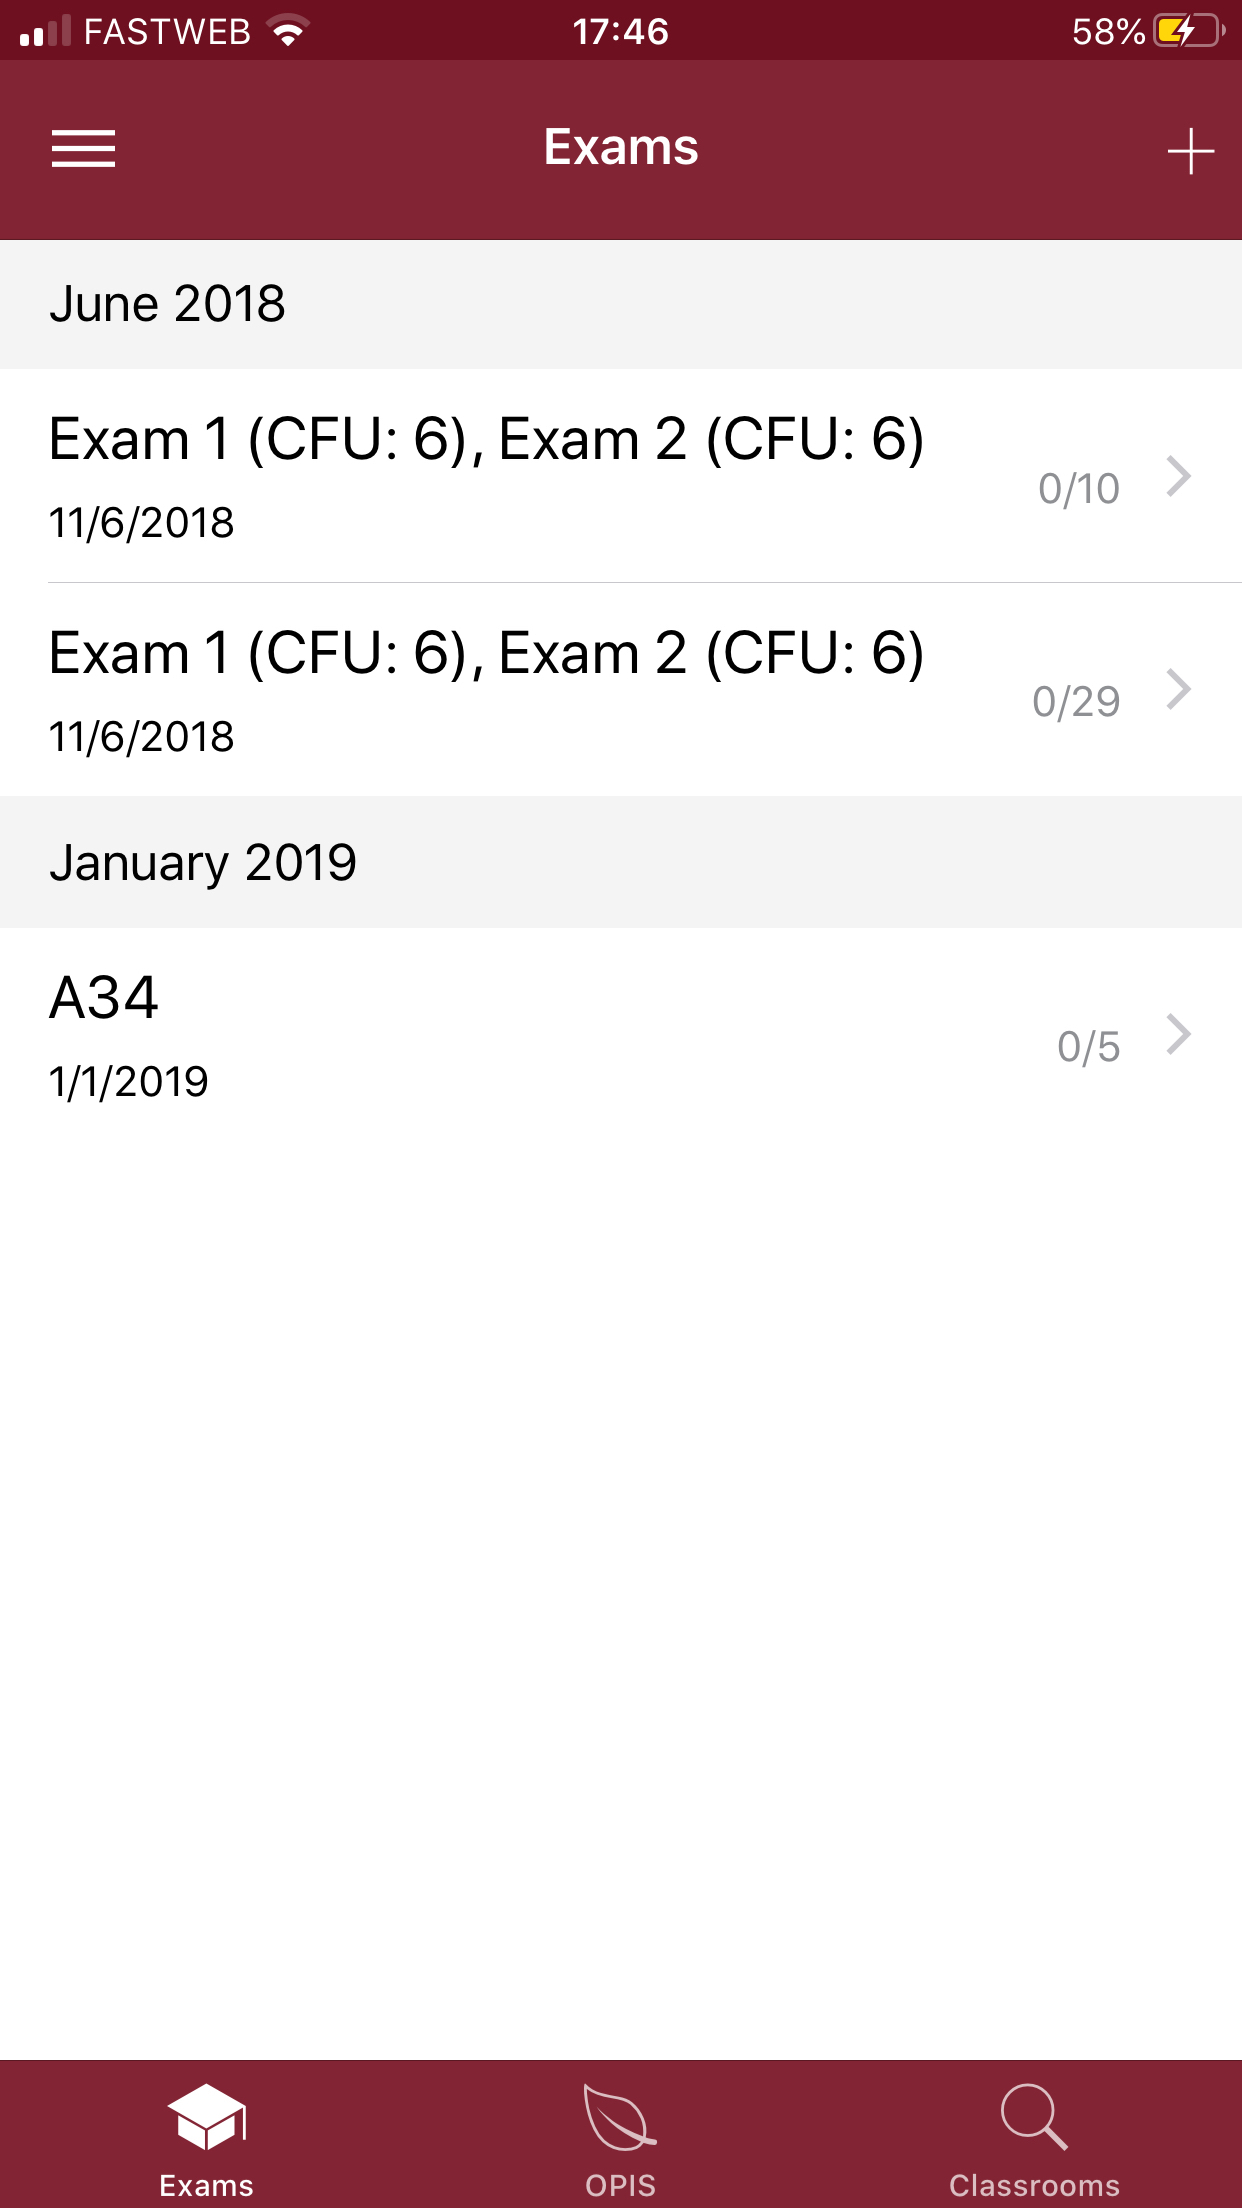
\includegraphics[width=0.5\linewidth]{ui-iterations/i/main}  
	  \caption{Put your sub-caption here}
	  \label{fig:sub-first}
	\end{subfigure}
	\begin{subfigure}{0.6\textwidth}
	  \centering
	  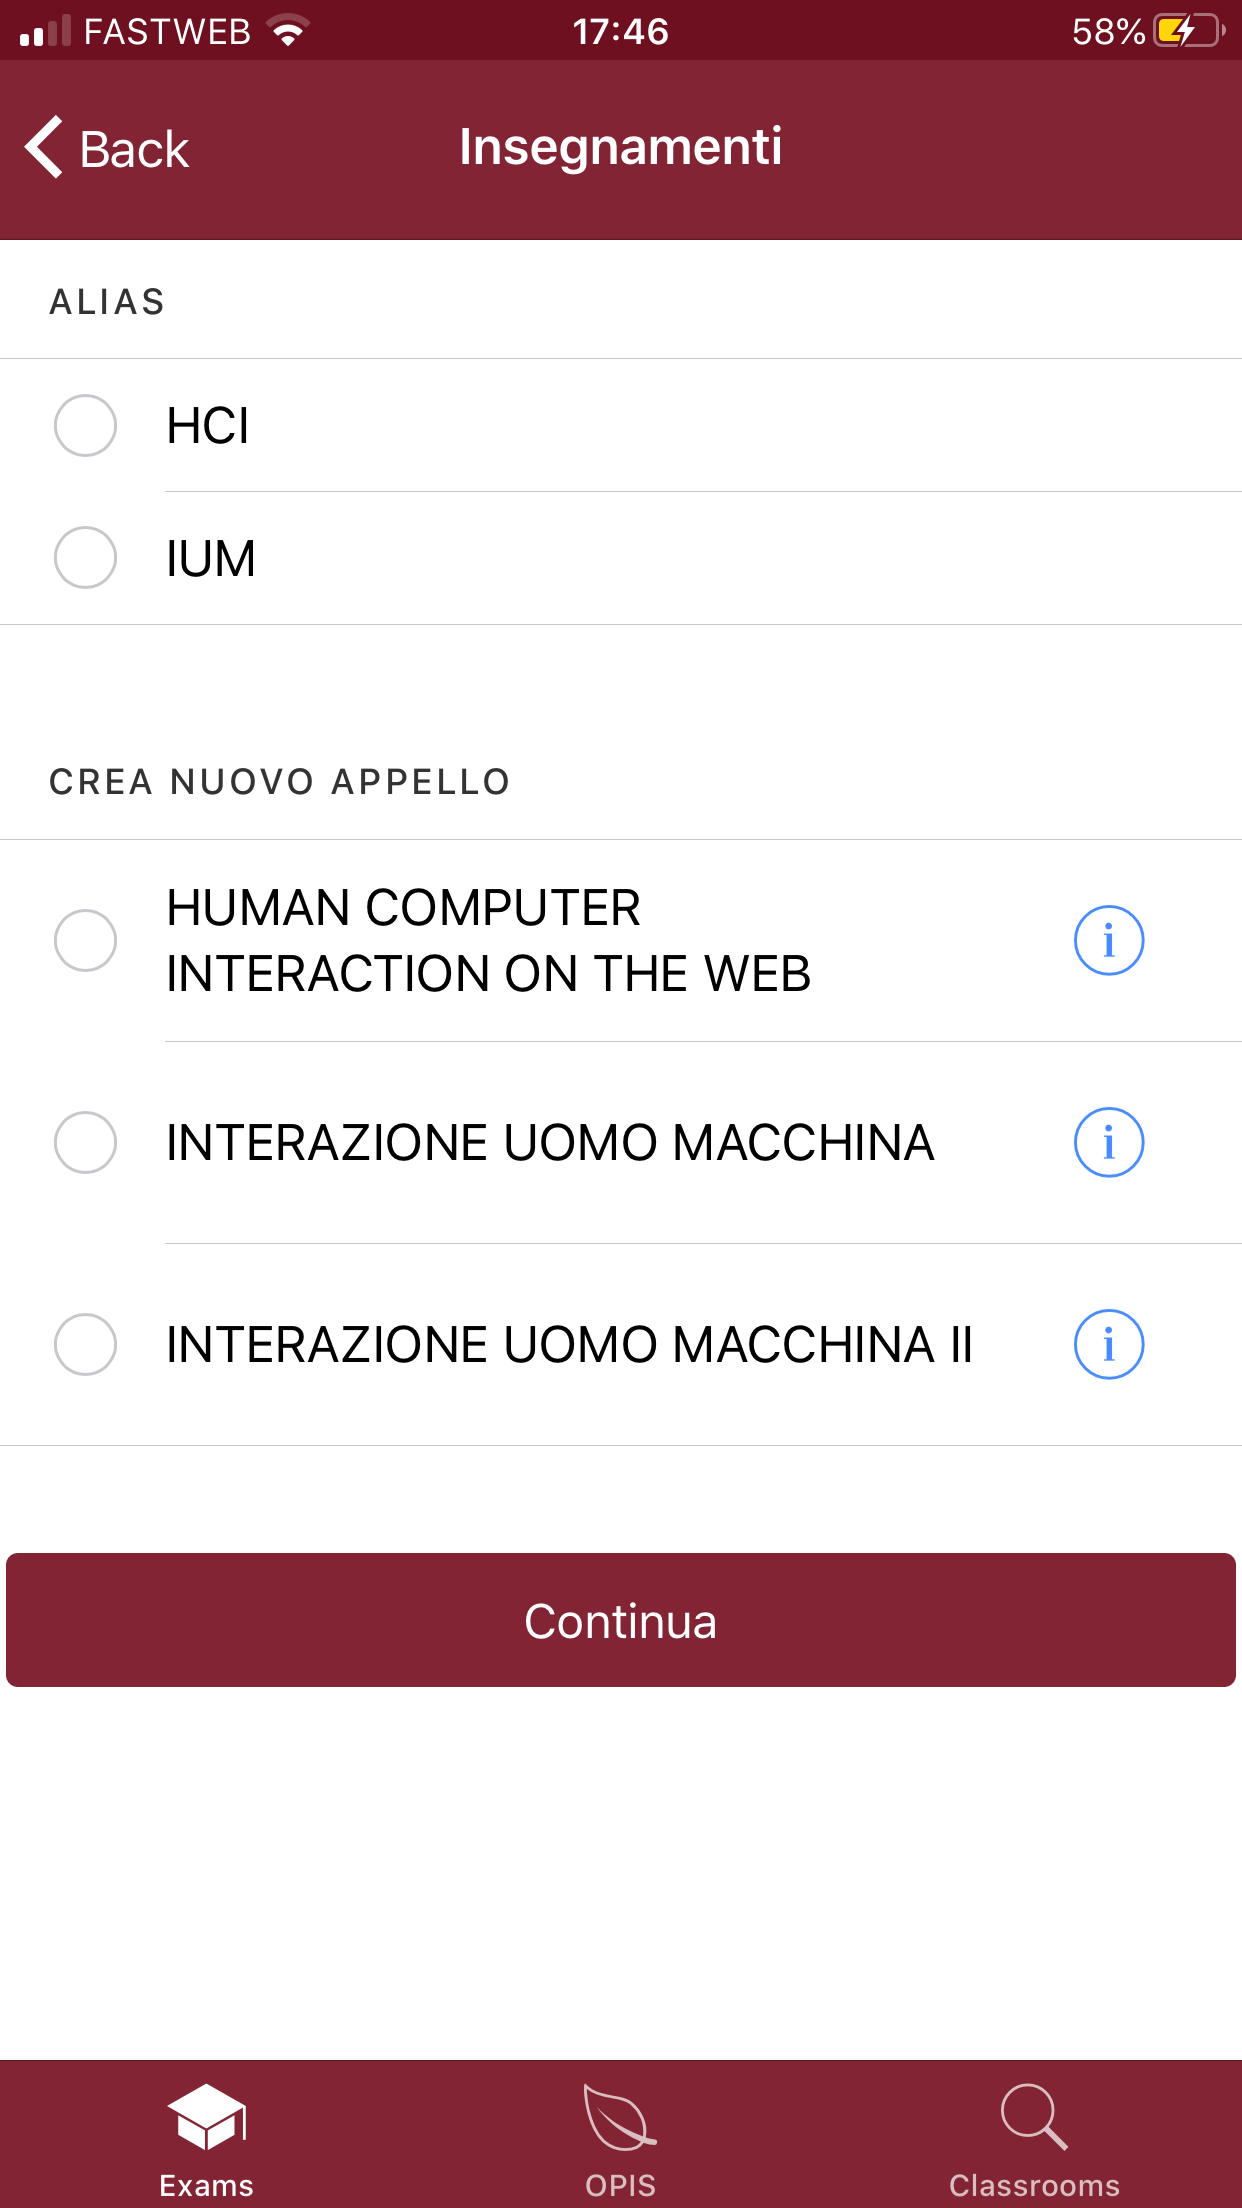
\includegraphics[width=0.5\linewidth]{ui-iterations/i/select-teaching}  
	  \caption{Put your sub-caption here}
	  \label{fig:sub-second}
	\end{subfigure}
	\begin{subfigure}{0.6\textwidth}
		\centering
		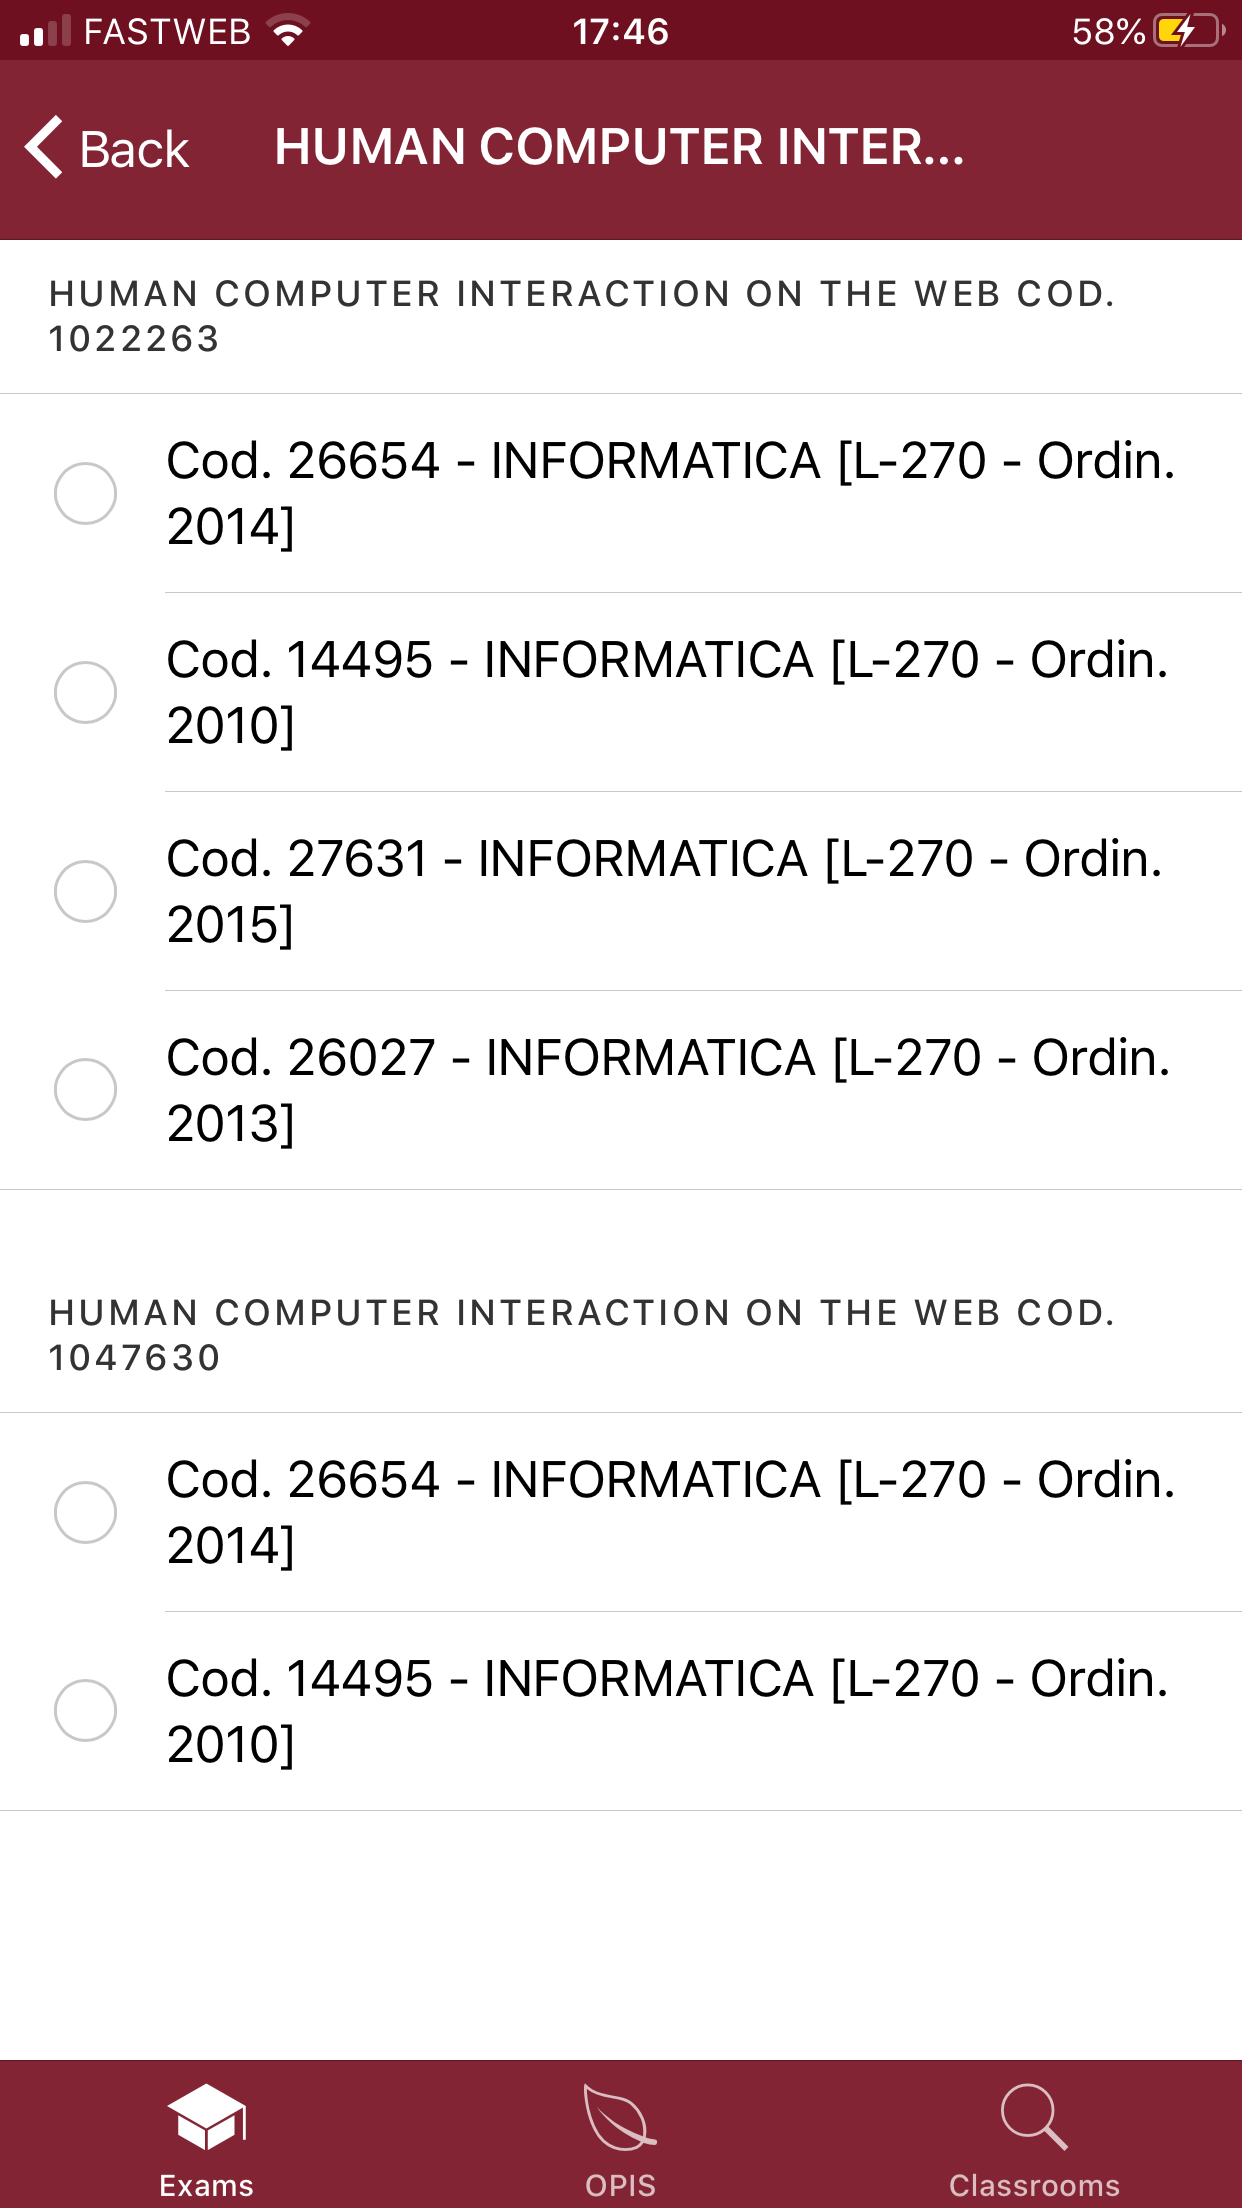
\includegraphics[width=0.5\linewidth]{ui-iterations/i/select-program}  
		\caption{Put your sub-caption here}
		\label{fig:sub-second}
	  \end{subfigure}
	  \begin{subfigure}{0.6\textwidth}
		\centering
		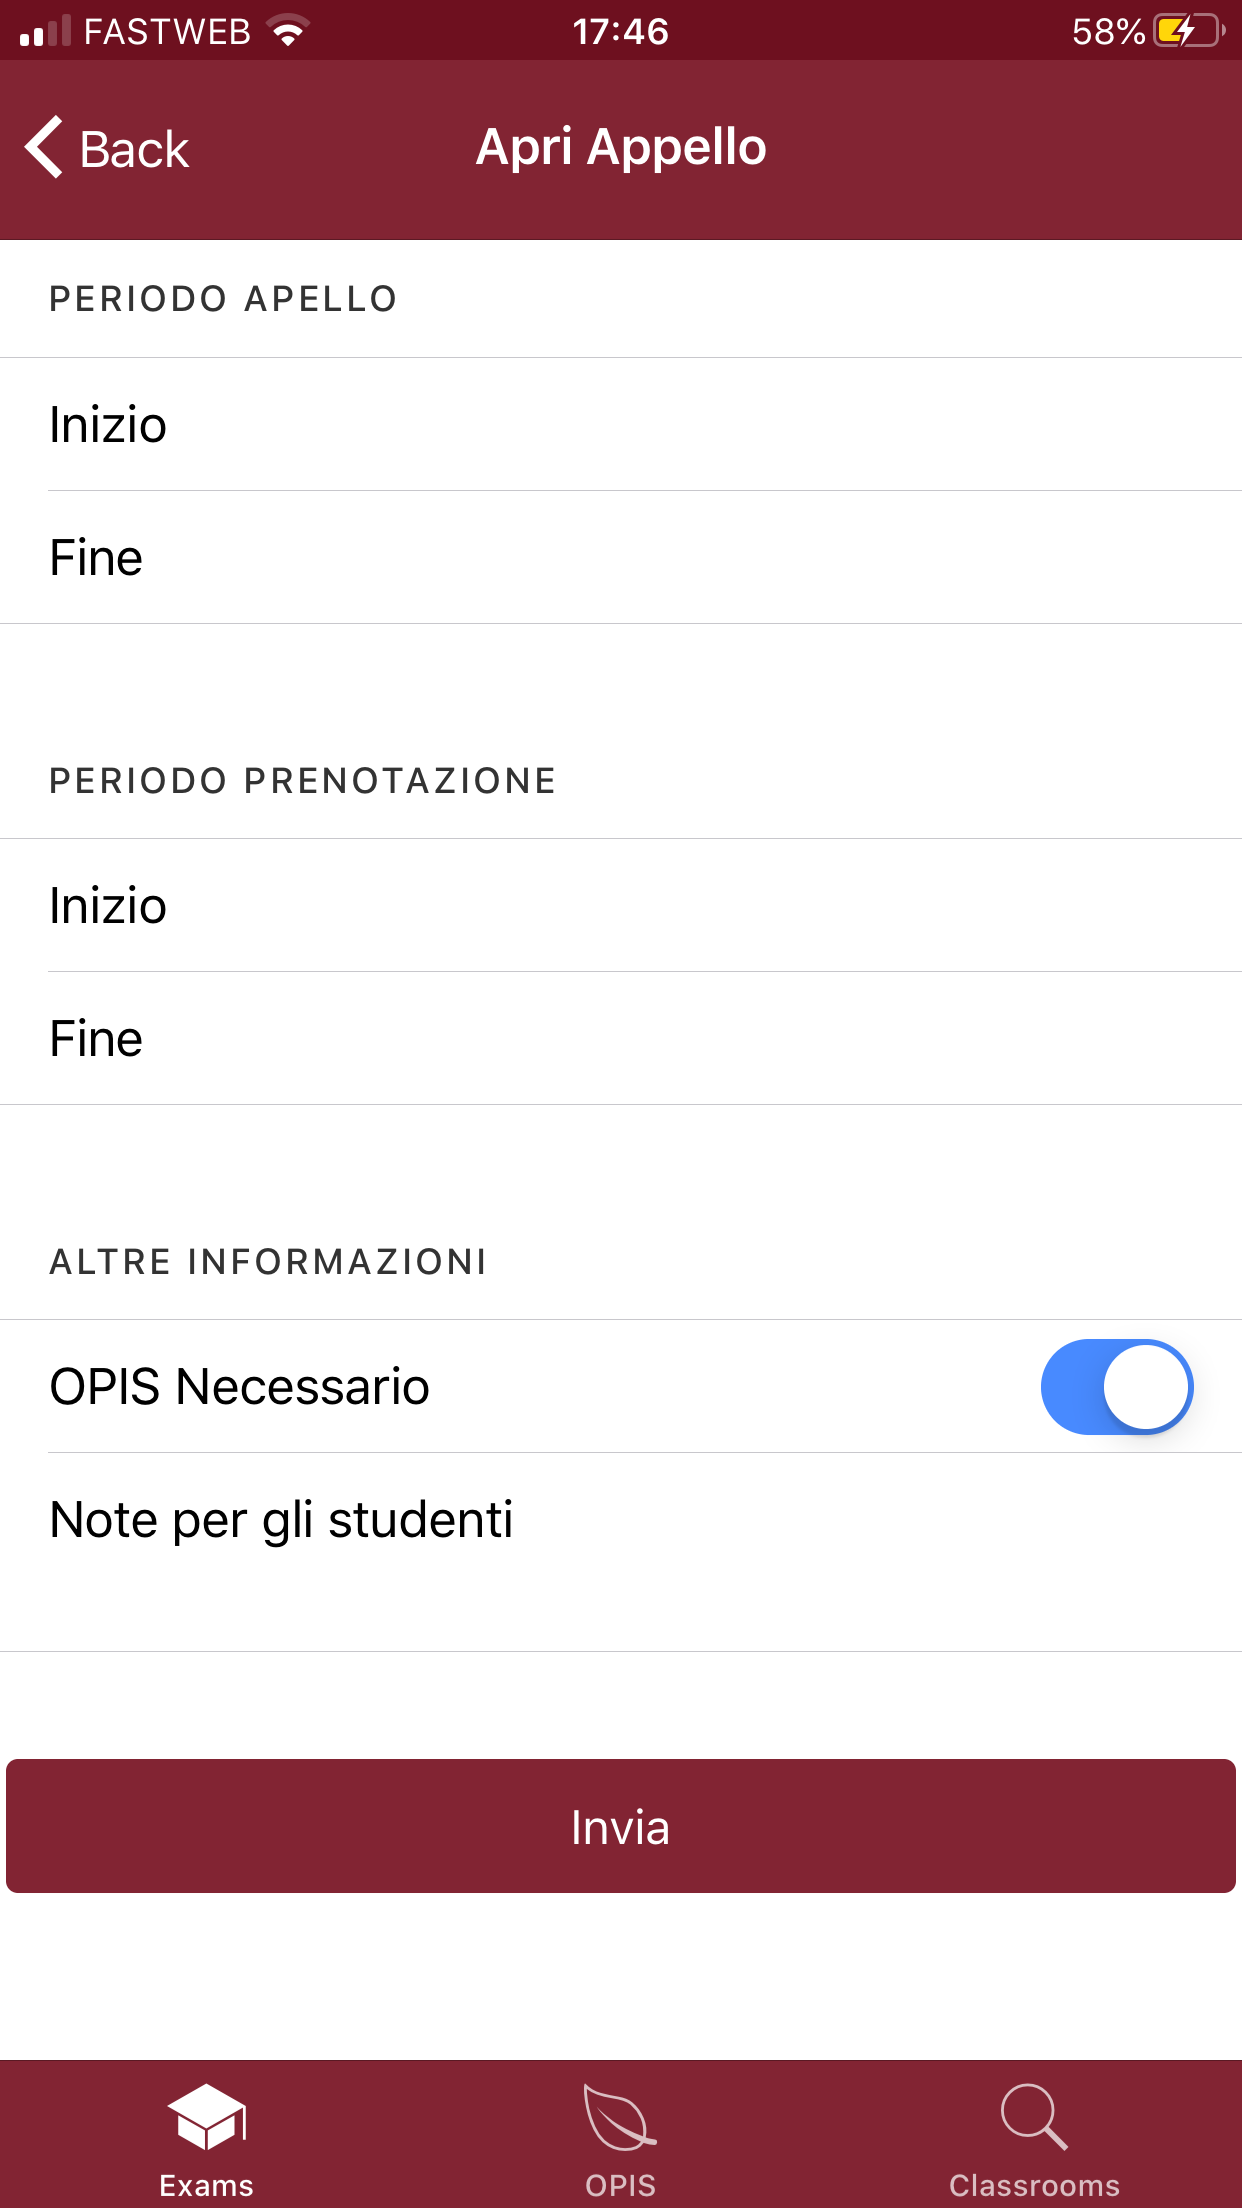
\includegraphics[width=0.5\linewidth]{ui-iterations/i/form}  
		\caption{Put your sub-caption here}
		\label{fig:sub-second}
	  \end{subfigure}
	  \begin{subfigure}{0.6\textwidth}
		\centering
		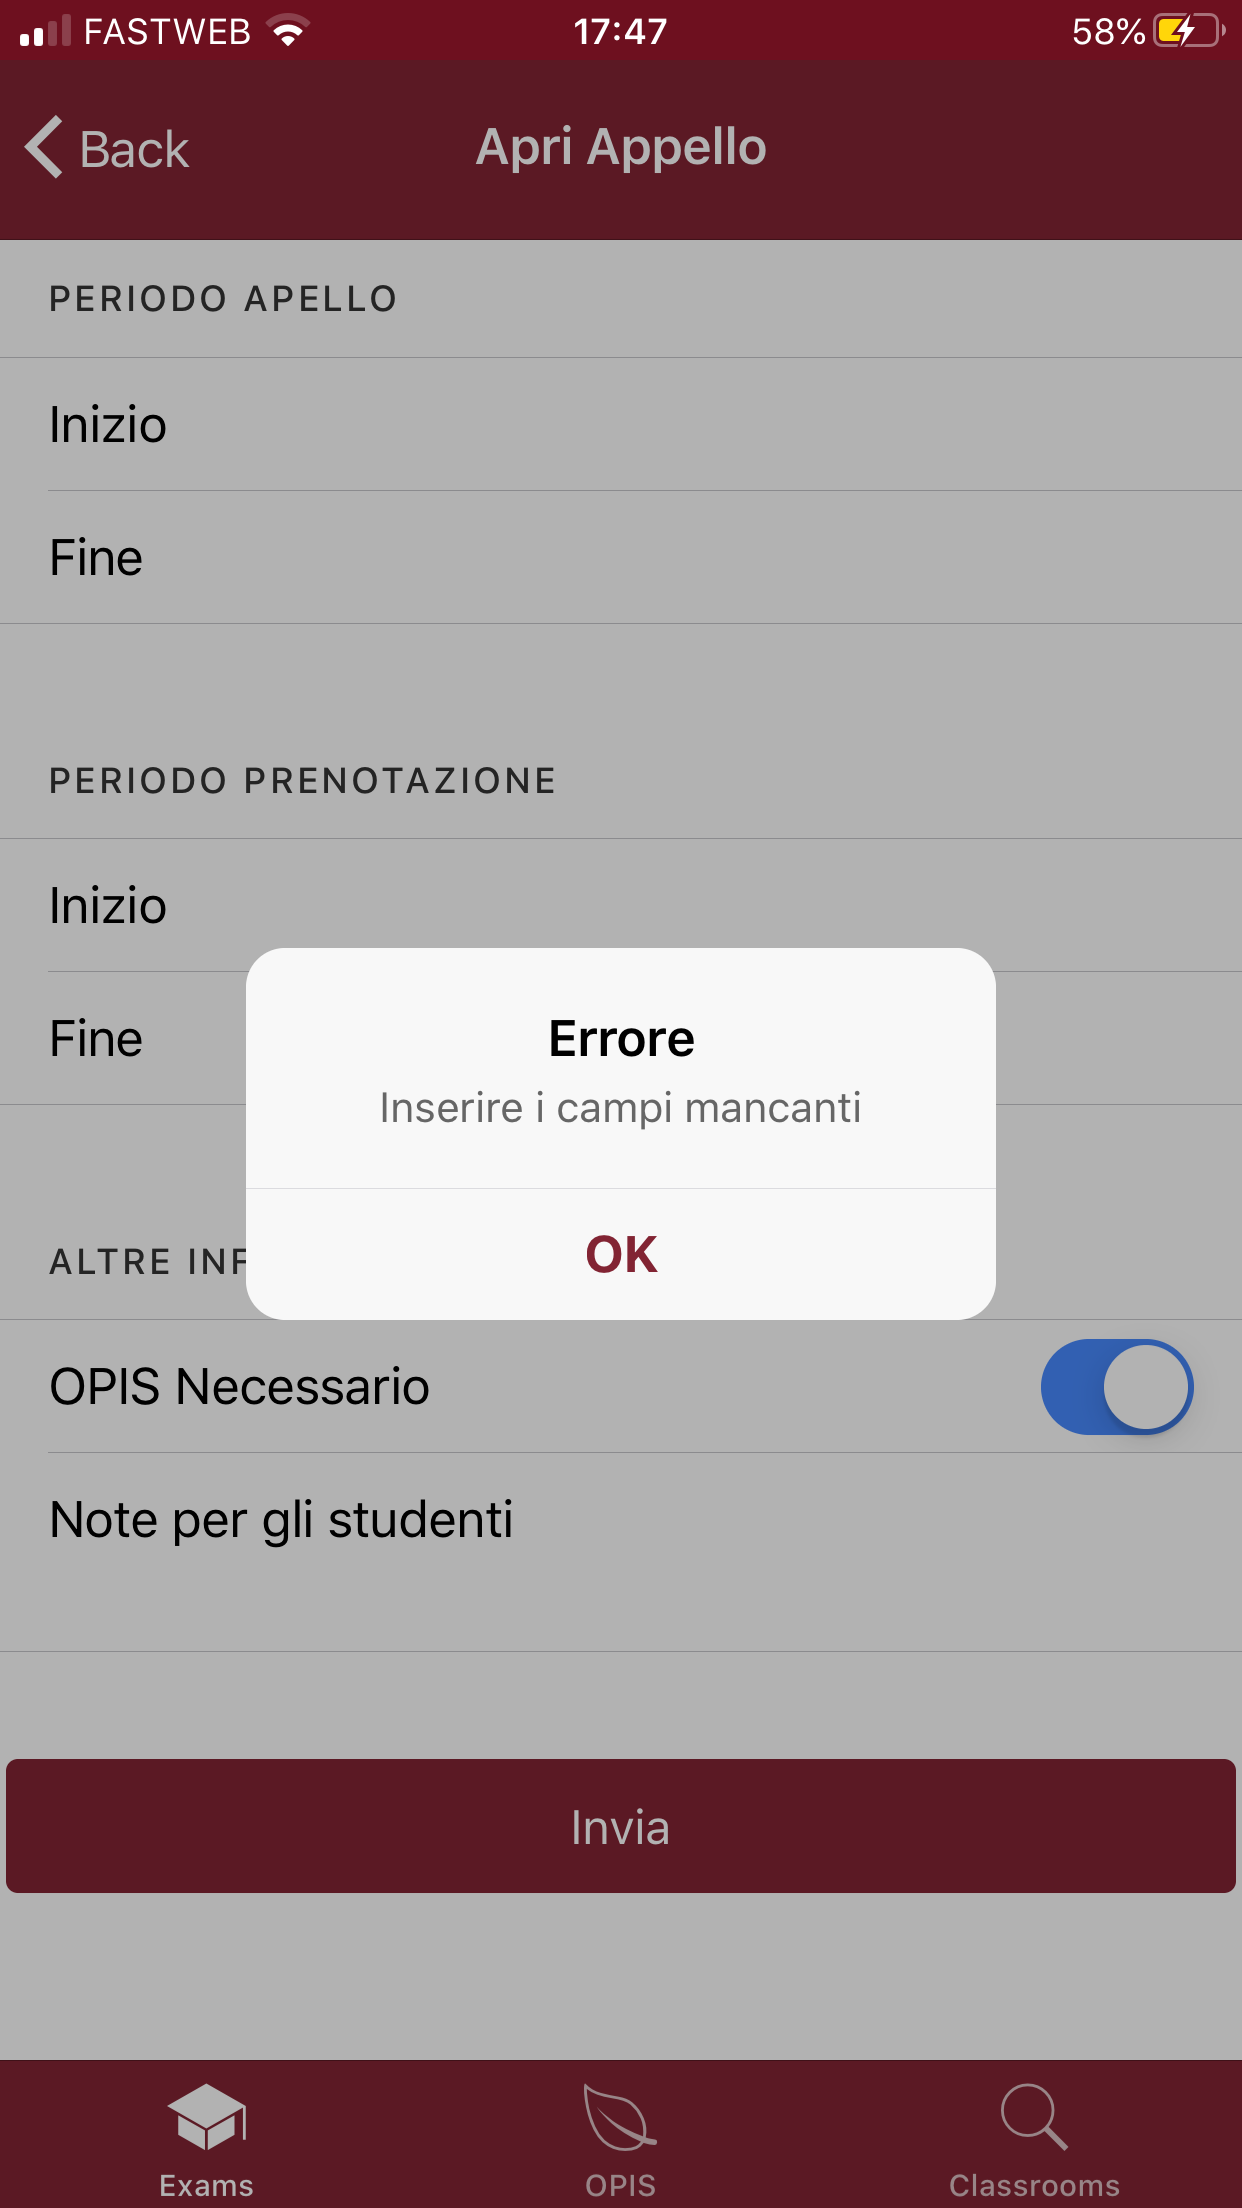
\includegraphics[width=0.5\linewidth]{ui-iterations/i/error-form}  
		\caption{Put your sub-caption here}
		\label{fig:sub-second}
	  \end{subfigure}
	  
	\caption{Prima iterazione}
	\label{fig:fig}
\end{figure}	

\subsection{Iterazione 2}
Il problema più grande della prima iterazione era il fatto che la prima view e la seconda (nella quale si inseriscono le date) non erano legate in alcun modo, questo costringe l'utente a ricordare le scelte fatte nella view precedente. Dato che la lista può essere complicata da gestire ed è importante aiutarlo a non fargli commettere errori, ho deciso di cambiare l'ordine della navigazione: la prima pagina infatti è stata spostata come prima view, con un bottone "Scegli insegnamenti" che porta alla pagina della scelta degli insegnamenti e degli alias. Quando questi vengono selezionati, si torna indietro e sopra al bottone di prima compaiono gli insegnamenti selezionati.

Altre modifiche all'interfaccia sono state quelle relative ai titoli delle navbar, che ora sono più inerenti, sono stati aggiunti dei messaggi di errore, il campo di testo ora è più chiaro ed ha un placeholder. In questa iterazione ho inoltre collegato le view al backend, dunque potevo lavorare su dei dati che strutturalmente rappresentavano i dati reali. Da qui ho implementato un meccanismo per sintetizzare la tabella degli insegnamenti, in cui parlerò più approfonditamente in \ref{sec:dev}.

Anche la grafica è cambiata, rendendola più simile a quella dell'aggiunta di un appuntamento sul calendario di iOS e Google. Non potendo fare più i test di usabilità, che hanno bisogno di essere fatti in presenza, mi sono affidato agli standard che hanno applicazioni più importanti. Infatti l'aggiunta di un appuntamento su un calendario non è tanto differente dall'apertura di un verbale: abbiamo infatti da gestire tre date in più rispetto ad un appuntamento, che in realtà si esaurisce nella giornata stessa, ma abbiamo da gestire in meno l'orario, il luogo, gli invitati e le etichette. Anche se, per utilizzare una metafora, si può pensare agli insegnamenti come degli invitati ed infatti il pulsante che permette di selezionare gli insegnamenti è molto simile a quello dell'aggiunta di persone all'evento.

Un altro miglioramento che è stato apportato è quello del compilamento automatico delle date. L'idea è quella di selezionare la data di inizio dell'appello e l'app, ricordando le date che sono state utilizzate precedentemente, prevede quali saranno quelle che l'utente inserirà, facendolo per lui. Infatti dalle interviste è emerso che i professori tendono a frammentarsi nel scegliere il numero di giorni dedicati all'appello e alle prenotazioni, ma la maggior parte è costante e utilizza sempre quelli. Dunque ho deciso di far ricordare all'applicazione le scelte fatte dall'utente in precedenza ed applicarle nella compilazione delle date.
Questo dovrebbe velocizzare di molto l'apertura di un verbale. % aggiungere eventuali feedback dati dalla beta

Infine, invece di utilizzare delle view, ho deciso di utilizzare dei modali per far sparire i tab a fine pagina. Questo impedisce all'utente di navigare all'interno dell'applicazione dopo aver iniziato l'apertura di un verbale, ma è ragionevole pensare che un utente non voglia farlo semplicemente perchè ho fatto in modo che tutto ciò che serve all'utente per aprire un appello è visibile nella pagina dedicata. Inoltre questo permette di risparmiare un po' di spazio per evitare lo scroll.

% analizzare la soddifacibilità dell'interfaccia con le euristiche proposte. Es. coerenza e standard per il fatto che si copia l'app di google e ios calendario, visibilità dello stato del sistema e riconoscere invece di ricordare tramite insegnamenti nella view principale, prevenzione degli errori tramite il collasso degli insegnamenti, design minimalista nascondendo i dettagli come quelli dei corsi associati agli insegnamenti e gli insegnamenti collassati in meno voci, efficienza d'uso tramite la compilazione automatica delle date, aiutare l'utente a diagnosticare gli errori tramite il ristrotturamento degli errori (poco chiari nella piattaforma desktop), corrispondenza tra il mondo reale e il sistema utilizzando sempre gli stessi termini per appello, insegnamento e corso. Libertà e controllo tramite la scelta dei corsi.

\begin{figure}[ht]
	\begin{subfigure}{0.6\textwidth}
	  \centering
	  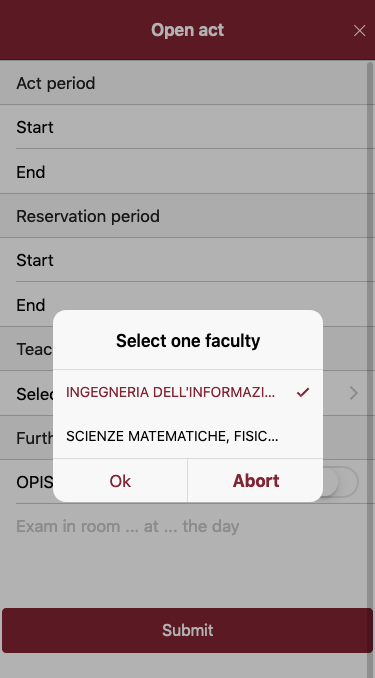
\includegraphics[width=0.5\linewidth]{ui-iterations/ii/select-faculty}  
	  \caption{Put your sub-caption here}
	  \label{fig:sub-first}
	\end{subfigure}
	\begin{subfigure}{0.6\textwidth}
	  \centering
	  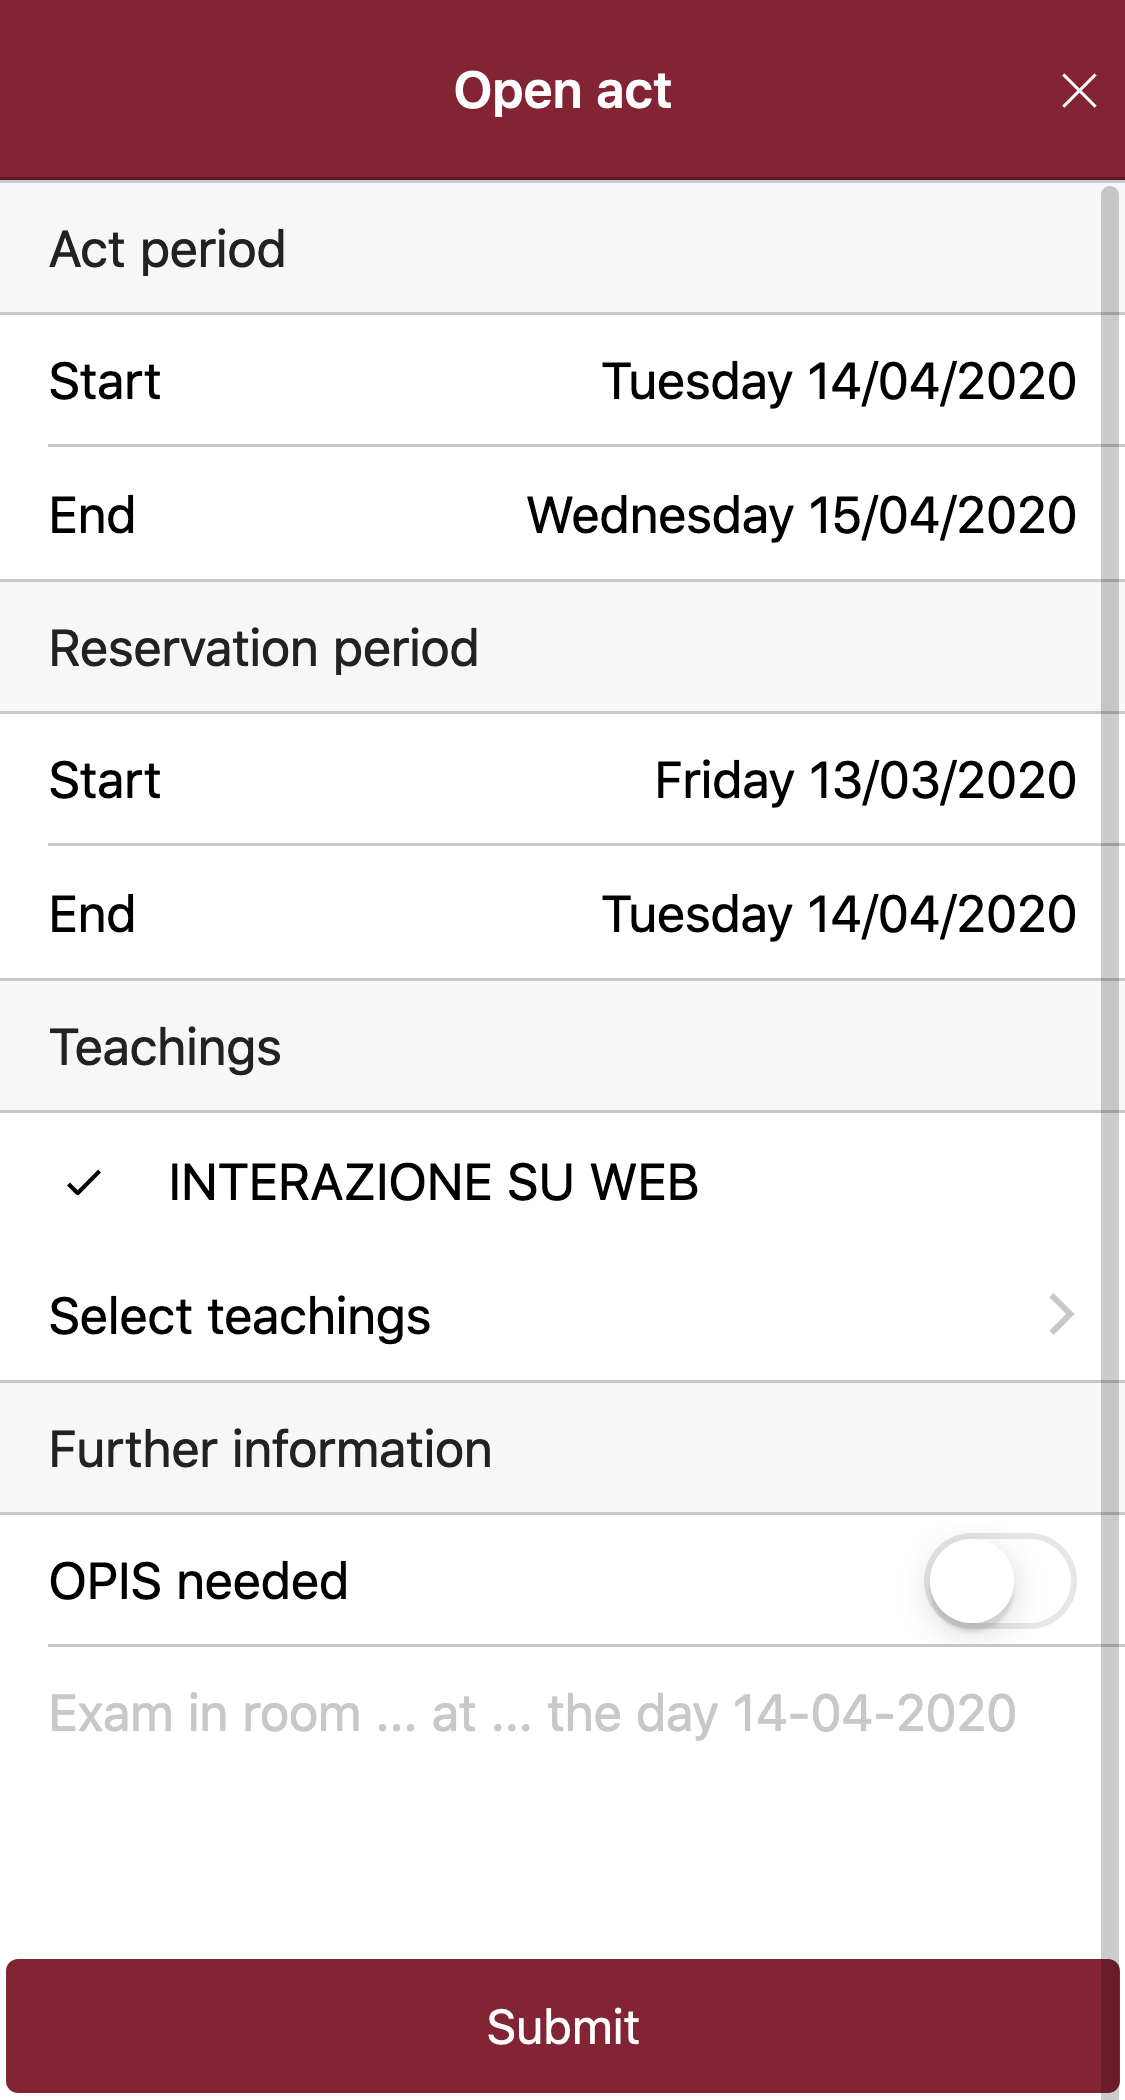
\includegraphics[width=0.5\linewidth]{ui-iterations/ii/form}  
	  \caption{Put your sub-caption here}
	  \label{fig:sub-second}
	\end{subfigure}
	\begin{subfigure}{0.6\textwidth}
		\centering
		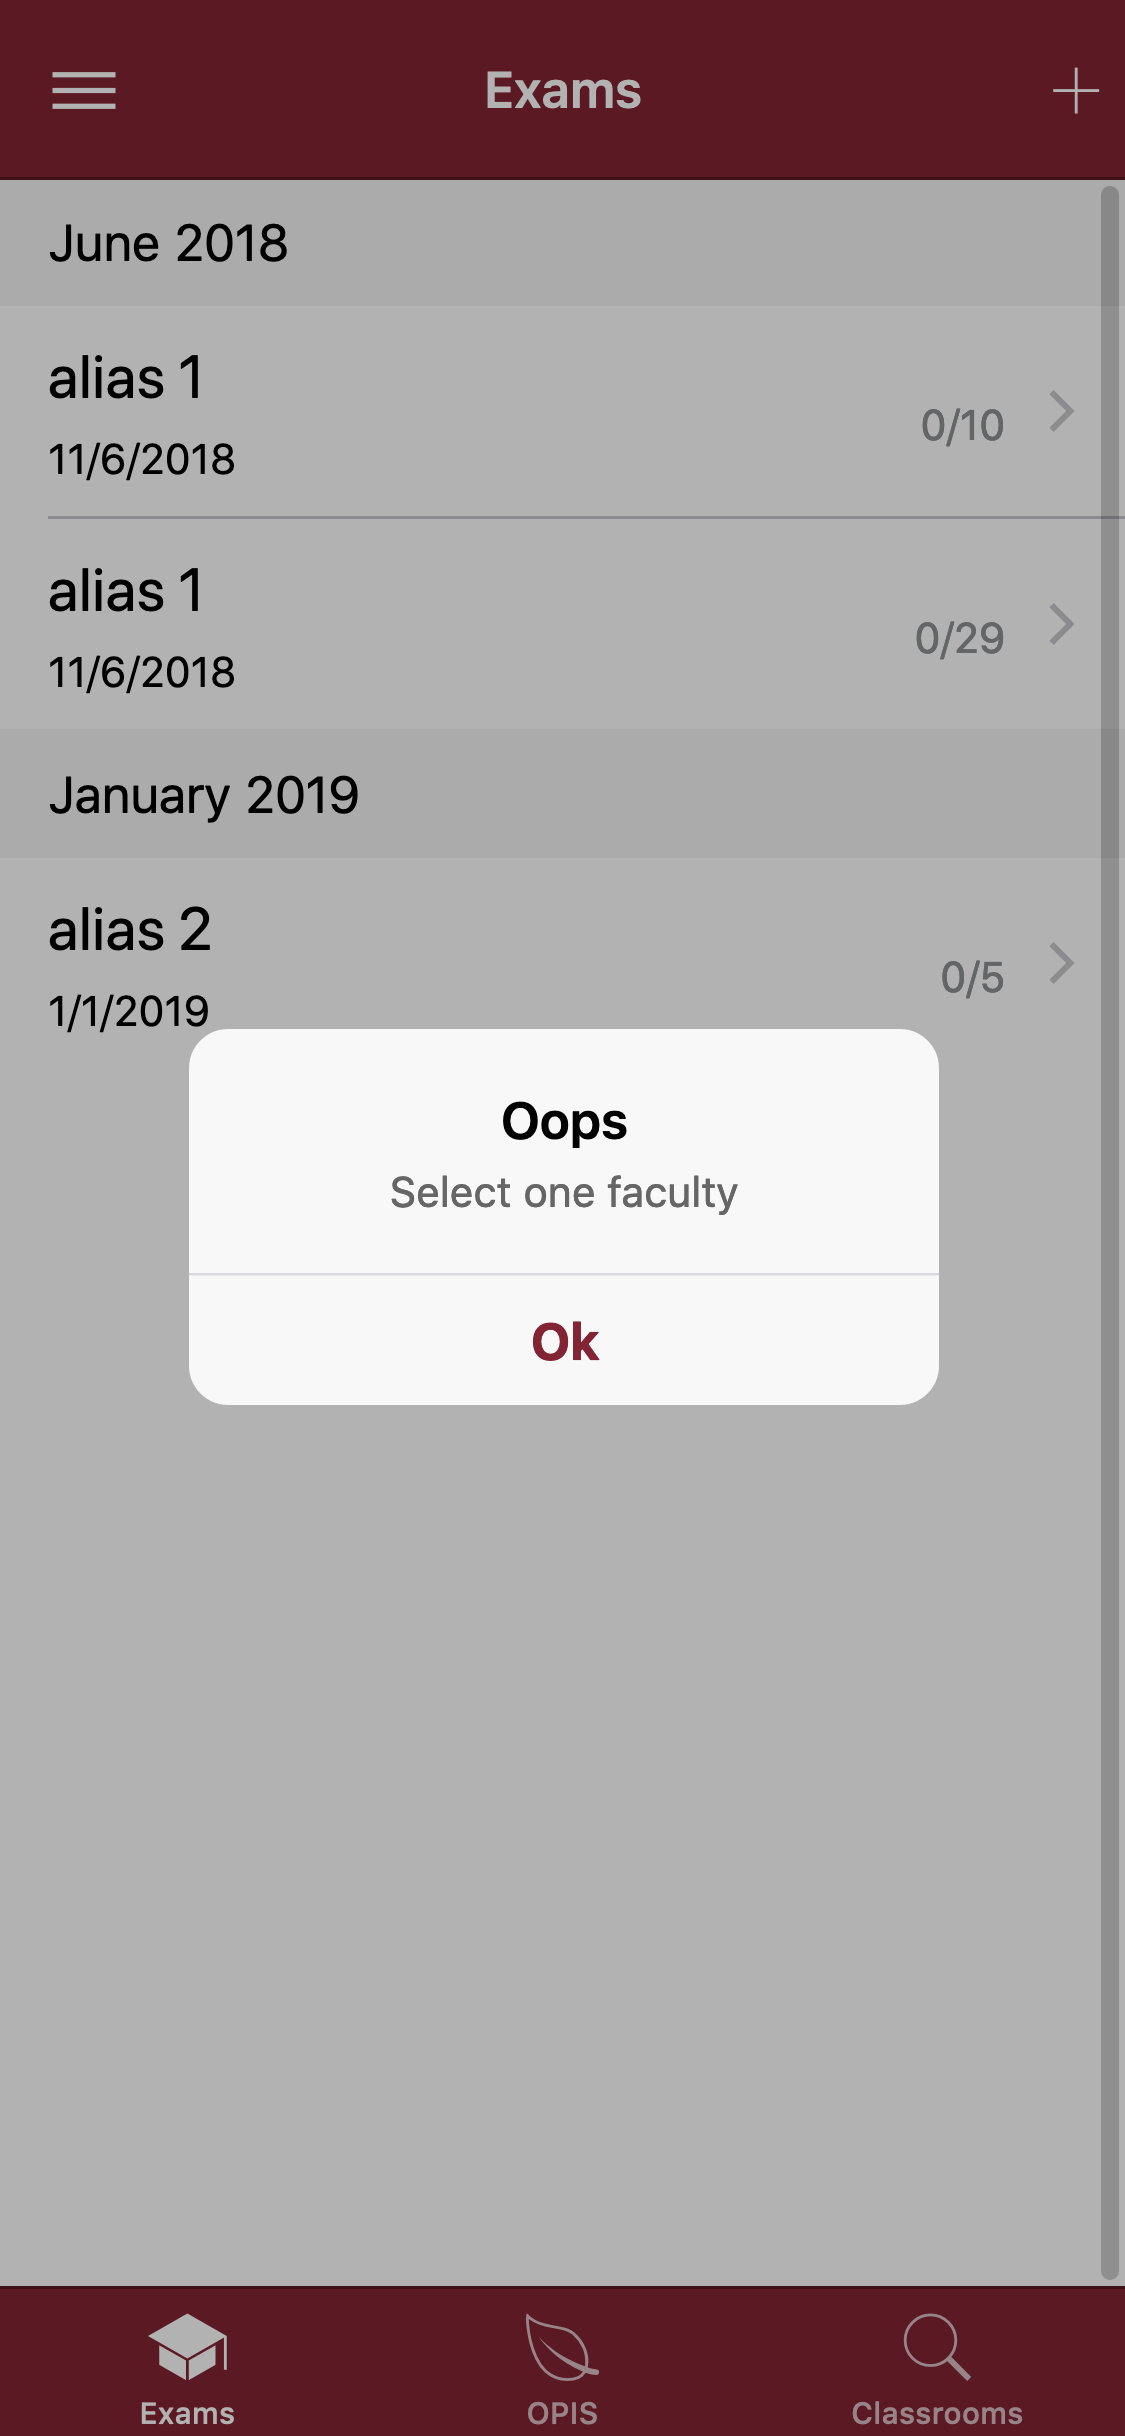
\includegraphics[width=0.5\linewidth]{ui-iterations/ii/error-faculty}  
		\caption{Put your sub-caption here}
		\label{fig:sub-second}
	  \end{subfigure}
	  \begin{subfigure}{0.6\textwidth}
		\centering
		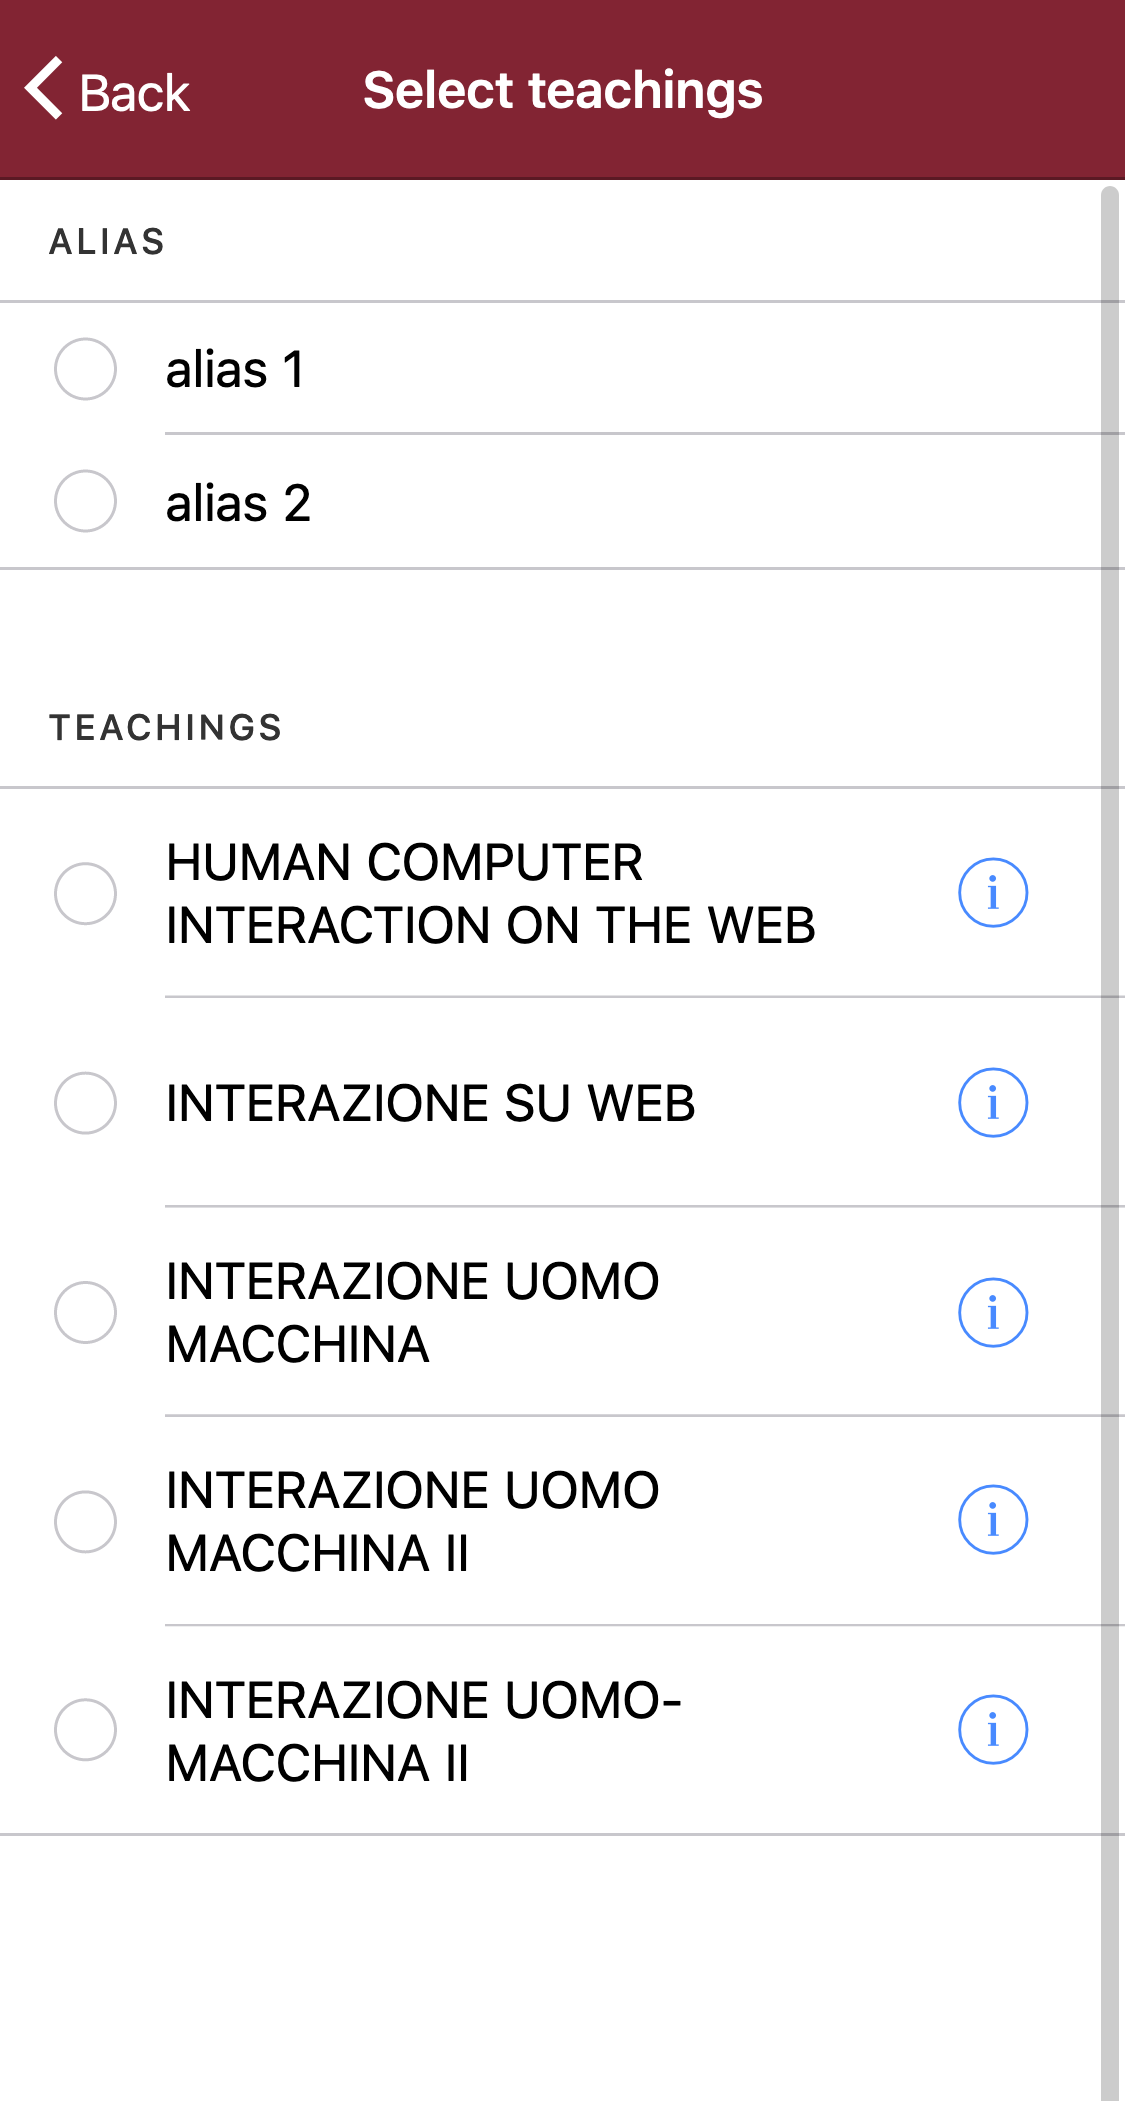
\includegraphics[width=0.5\linewidth]{ui-iterations/ii/teaching-list}  
		\caption{Put your sub-caption here}
		\label{fig:sub-second}
	  \end{subfigure}
	  
	\caption{Seconda iterazione}
	\label{fig:fig}
\end{figure}

\subsection{Iterazione 3}


\section{Implementazione}
\label{sec:dev}
%inserire qualche snippet, parlare di come si sono "collassati" gli insegnamenti, come si passano i dati tra le view, ecc...


\chapter{Conclusioni}
\label{ch:4}

\backmatter
\phantomsection
\begin{thebibliography}{17}

\bibitem{ref:mit}
Tratto da MIT:
\url{http://web.mit.edu/6.813/www/sp18/classes/09-more-learnability/#consistency}

\end{thebibliography}

\end{document}